\documentclass[12pt,a4paper]{article}
\usepackage{amsmath}
\usepackage{mathrsfs}
\usepackage{cancel}
\usepackage{color}
\usepackage{circuitikz}
\usepackage{url}
%
%Nog iets over die dyes 
%
% Cal150, sigma50, sigma150
% Jsigma(50-150)
% Jcal(50:10:150)
% daarna: misschien meer stappen (55:10:145)
% optimize, eerst voor sigma, daarna voor JCal.
% Misschien beter om ode's the optimizen en dan sigma?


%H = hessian(J, m)
%eig = H.eigendecomposition(n=30)

%dJdm = Jhat.derivative()[0]
%H = Jhat.hessian(dm)[0]
\title{Inversion based on simultaneous observations of voltage and calcium concentration}
\author{Joanneke E Jansen}
\begin{document}

\maketitle
\section{Introduction} \label{Introduction}
In this report, we will investigate an inverse problem based on simultaneous observations of voltage and intracellular calcium concentration. Mathematically, inversion means the computation of the most plausible values of not directly observable parameters using a set of measurements. The classic technique to estimate electro-physiological cardiac parameters is patch clamping. With patch clamping, the transmembrane voltage of a single cell can be precisely measured over time. An alternative for the time and labour intensive patch clamping technique could be optical mapping, with which voltage and calcium waves of a cluster of cells can be measured simultaneously \cite{Lee2012}. The monodomain model is a commonly used model to simulate cardiac electro-physiology. Here, we will look if we can use this monodomain model to infer parameters based on voltage and intracellular calcium measurements, breaking the single cell tradition. As a motivating example, we will model the behaviour of monolayers of human incuduced pluripotent stem cell-derived cardiomyocytes (iPSC-CMs). In recent years, there has been a large interest in iPSC-CMs as a tool for drug screening and disease modelling and more efficient techniques for doing so are needed.

\subsection{Human induced pluripotent stem cell-derived cardiomyocytes (iPSC-CMs)}
Human induced pluripotent stem cell-derived cardiomyocytes (iPSC-CMs) provide a promising platform for studying cardiac cells in vitro. In 2007, it was first described how iPSCs can be made by reprogramming somatic cells \cite{Takahashi2007}. Since then, there has been a large interest in using those cells for drug safety screening and disease modelling \cite{Sallam2016}. Human iPSCs are self-renewing, patient-specific, and can be differentiated to cell types such as cardiomyocytes, hepatocytes and neurons \cite{Rajamohan2013}. In recent years, the techniques for efficiently producing homogeneous populations of iPSC-CMs  have greatly improved. However, the production process of iPSC-CMs is still very expensive in comparison to most \textit{in vitro} models. The largest limitation of the currently produced iPSC-CMs is their immature, foetal phenotype, although improvements in maturity are still being made \cite{Denning2016}. 
\subsection{Optical mapping}
There are several techniques to study the electrophysiology of iPSC-CMs. The method most commonly used is patch clamping. With this technique the transmembrane potential $v$ of a single cell can be precisely measured, but patch clamping is time and labour intensive and thus precludes efficient large-scale screening. An alternative to patch clamping is optical mapping \cite{Denning2016}. With optical mapping, the transmembrane potential $v$ can be measured with a high spatial and temporal resolution. Although optical mapping methods tend to slightly overestimate the duration of action potentials, the shape of the measured action potential is similar for both techniques \cite[Figure 2]{Leyton2014}. Unlike the invasive patch clamping technique, optical mapping allows for action potential measurements of large cell populations and sequential measurements of the same groups of cells. Furthermore, it is possible to not only measure the transmembrane potential, but also the intracellular calcium concentration $[Ca]_i$, at the same time \cite{Lee2012}. 
%Zhu2017, microarray, also spatial variation (maar geen high reso, al weet ik niet of dat erg is)
%Bedut 2016 for microarrays
\subsection{Overview}
The aim of this report is to investigate the possibilities of parameter estimation of iPSC-CMs based on data obtained by optical mapping. In particular, we are interested to see what extra information can be inferred from the high spatial resolution and simultaneous calcium and voltage recordings, in contrast to the single cell voltage recordings obtained by patch clamping. We will model the behaviour of a monolayer of iPSC-CMs with the classic monodomain equations, which we will introduce in Section \ref{The monodomain model}. To model the cell membrane dynamics, we will use the Paci2013 cell model. The Paci2013 cell model is specifically developed for the simulation of iPSC-CMs action potentials and is based on data obtained on iPSC-CMs \cite{Paci2013, Ma2011}. Due to the already mentioned immature phenotype of currently produced iPSC-CMs, there is a lot of variability in the action potential shape of different cells, even if they are part of the same cell cluster \cite{Blazeski, Zhu2016}. Therefore, the predictive value of the Paci2013 and other cell models will be limited and our investigation must be seen as a proof of concept. The development of iPSC-CMs technologies is rapid and produced iPSC-CM clusters are hoped to become more homogeneous and similar to mature cardiomyocytes in the near future \cite{Denning2016}. 
%In Section \ref{The monodomain model}, we introduce the monodomain model and in Section \ref{The Paci2013 cell model} the Paci2013 model. After that, we introduce a basic test case in section \ref{Basic test case} and \ldots
\section{Mathematical models} \label{Mathematical models}
\subsection{The monodomain model} \label{The monodomain model}
The monodomain equations are given by 
\begin{eqnarray} \label{eq:a}
\frac{\partial \mathbf{s}}{\partial t}= \mathbf{F}(\mathbf{s},v), \qquad \mathbf{x} \in H, \\
\frac{\partial v}{\partial t} + I_{ion}(v,\mathbf{s}) =\nabla \label{eq:b} \cdot(\mathbf{M}\nabla v) + I_s,\qquad \mathbf{x} \in H, \\ \label{eq:c}
\mathbf{n}\cdot (\mathbf{M}\nabla v)=0, \qquad \mathbf{x} \in \delta H,
\end{eqnarray}
with $v(\mathbf{x},t)$ the transmembrane potential (in mV), $H$ the domain, $\delta H$ the boundary of $H$, $\mathbf{n}$ the outward pointing normal of the boundary, and with $I_s$ the prescribed input current (in mV/ms) and $I_{ion}$ the ionic current across the membrane (in mV/ms), both scaled by the cell membrane capacitance (in $\mu$F/(mm$^2$)). 
Equation \eqref{eq:a} is a system of ODE's that models the membrane dynamics. There exist many different cell membrane dynamics models with varying degrees of complexity that can be used to specify $I_{ion}$, $\mathbf{F}(\mathbf{s},v)$ and the state variables $\mathbf{s}$, see the CellML repository \cite{cellml} for an overview of different types of models. In this report, we will use the Paci2013 cell model, that is specifically developed to model the electrophysical behaviour of iPSC-CMs \cite{Paci2013}. We will introduce the Paci2013 cell model in the next section.\\ Finally, $\mathbf{M}$ is a conductivity tensor (in mm$^2$/ms), that satisfies 
\begin{equation}
\mathbf{M}=\frac{\alpha}{1+\alpha}\mathbf{M}_i,\label{eq:d}
\end{equation}
with $\mathbf{M}_e=\alpha \mathbf{M}_i$. Here, $\mathbf{M}_e$ and $\mathbf{M}_i$ are the extracellular and intracellular conductivities (in mm$^2$/ms), divided by the product of the membrane capacitance (in $\mu$F/(mm$^2$)) and the cell membrane area-to-volume ratio (in 1/mm). By assuming that there exists a $\alpha$ such that $\mathbf{M}_e=\alpha \mathbf{M}_i$ the monodomain equations can be derived from the more complicated bidomain equations \cite[p. 566-568]{KeenerII}.
\subsection{The Paci2013 cell model} \label{The Paci2013 cell model}
The Paci2013 model consists of 18 ODEs and is of Hodgkin-Huxley type (see \cite[p. 195-215]{KeenerI} for an introduction to the Hodgkin-Huxley equations). The ionic current $I_{ion}$ is a sum of twelve different ion channel type currents:
\begin{eqnarray}
I_{ion}=I_{Na}+I_{CaL}+I_f+I_{K1}+I_{Kr}+I_{Ks}+ \\
I_{to}+I_{NaCa}+I_{NaK}+I_{pCa}+I_{bNa}+I_{bCa}.
\end{eqnarray}
An ion channel current $I_k$ is typically of the form 
\begin{equation}
I_{k}=g_k m_k^{p_k}\ldots h_k^{q_k}(u_m-u_k),
\end{equation}
where $g_k$ is the maximum conductance $g_k$ (in $\mu$S/$\mu$m$^2$), $u_k$ (in mV) the Nernst potential and $m_k$, $h_k \ldots$ are a certain number of voltage and time dependent gating variables. Each ion channel type has different types of gating variables. The Paci2013 model contains ODEs for thirteen different ionic gating variables. Apart from the ionic gating variables and an inner calcium dynamics gating variable, the state variables of the Paci2013 model also include the intracellular sodium and calcium, and the sarcoplasmic reticulum calcium concentrations $[Na]_i, [Ca]_i$ and $[Ca]_{SR}$ \cite{Paci2013}. The estimation of the model parameters was mainly based on patch clamp iPSC-CM data from \cite{Ma2011}. The iPCS-CMs studied by \cite{Ma2011} showed atrial-, nodal-, and ventricular-like action potentials. The Paci2013 model contains of two sets of parameters: one to simulate ventricular-like cells and one to simulate atrial-like cells. 
%Although AL cells are present in in vitro prepara- tions, they are a less common phenotype compared with the VL ones, and they are rarely used for drug tests. Paci2015

%
\section{Basic test case} \label{Basic test case}
%For our test case, we take a square of $5$ mm $\times\: 5$ mm as our domain $H$. We will use the Grandi cell model to model the membrane kinetics \cite{Grandi}. We solve our test case with the \url{splittingsolver} module from the cbcbeat Python package \cite{cbcbeat}\footnote{This electrophysiology solver package is based on the FEniCS Project software \cite{fenics} and the dolfin-adjoint software \cite{dolfin-adjoint}} with the default parameter values and default initial conditions for $v$ and $s$. The \url{splittingsolver} solves the monodomain PDE system and its coupled cell membrame dynamics ODE system separately, using the operator splitting scheme as described in \cite{Sundnes}. We take typical values $\sigma_l=0.15$ and $\sigma_t=0.02$ (in mS/mm) for the longitudinal and tangential conductivity respectively and take $C_m=0.2$ for the membrane capacitance (in $\mu$F/(mm$^2$)) and $\beta=200$ for the cell membrane area-to-volume ratio (in 1/mm) \cite{Roth}, data from \cite{Plonsey1882, Plonsey1984}.
%We apply a stimulus of $10$ mV/ms over 0.25 mm$^2$ in the centre of the square from $t=0$ to $t=3$ ms. In Figure \ref{fig:1}, we show a heat map of $v$ at $t=5, 15, 40$ and $80$ ms. In Figure \ref{fig:2}, we show a heat map of $[Ca]_i$ at the same times. This variable is one of the 37 state variables $\mathbf{s}$ of the Grandi cell model and measures the cytosolic calcium concentration \cite{Grandi}. In Figures \ref{fig:3} and \ref{fig:4}, we plotted $v$ and $[Ca]_i$ (in $\mu$M) over time, both at a point at the centre of the domain (in blue) and at a point at the left lower edge (in green).
%
%%4 V during 3 ms p. 1487, Lee-peter-2011, misschien kleiner domein nemen?
%
%\begin{figure}
%
%\begin{minipage}{0.47\textwidth}
% \textbf{(a)} 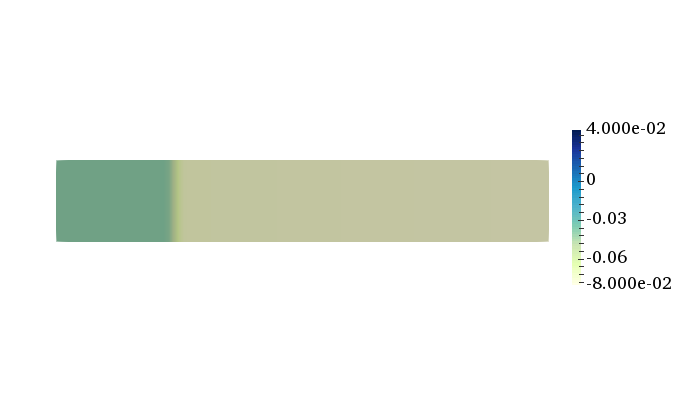
\includegraphics[trim=9cm 0cm 2cm 0cm, clip=true, width=0.9\linewidth]{v5}
%      \textbf{(c)} 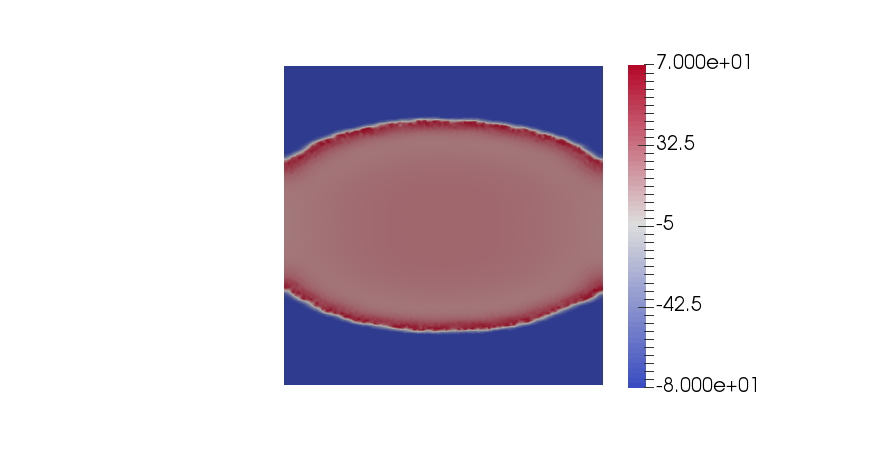
\includegraphics[trim=9cm 0cm 2cm 0cm, clip=true, width=0.9\linewidth]{v40}
%    \end{minipage}
%    \begin{minipage}{0.47\textwidth}
%  \textbf{(b)} 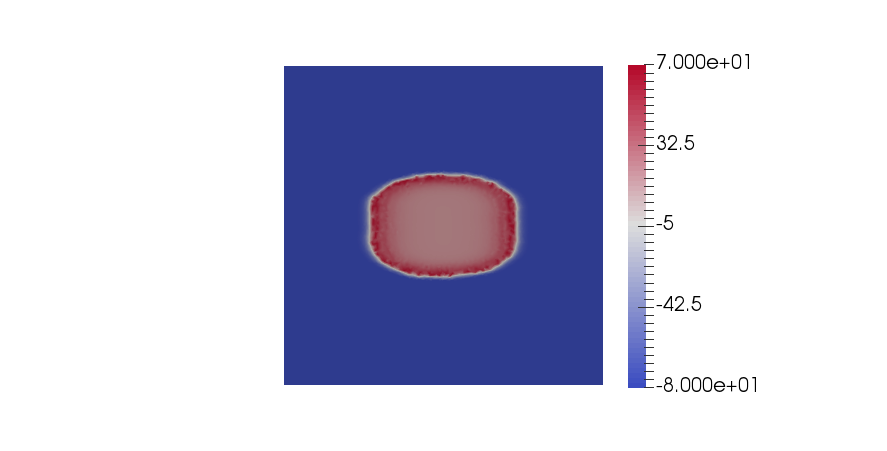
\includegraphics[trim=9cm 0cm 2cm 0cm, clip=true, width=0.9\linewidth]{v15}
%  \textbf{(d)} 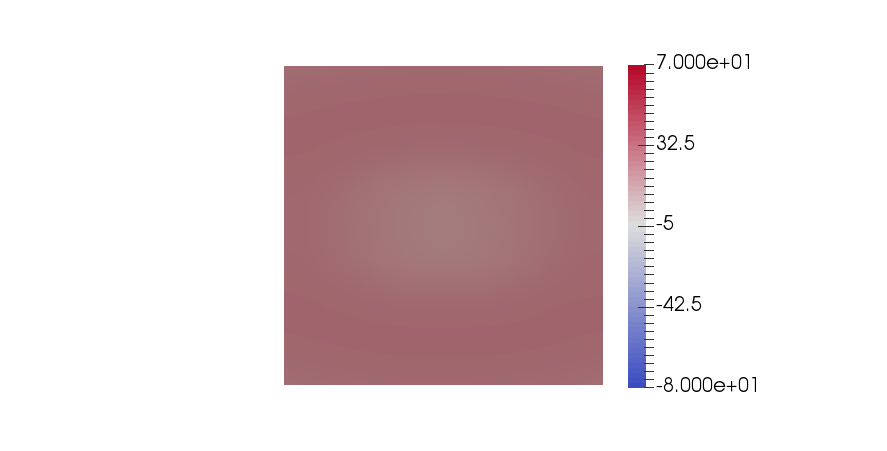
\includegraphics[trim=9cm 0cm 2cm 0cm, clip=true, width=0.9\linewidth]{v90}
%    \end{minipage}
%    \caption{Heat maps of $v$ (in mV) of our basic test case at \textbf{(a)} $t=5$ms, \textbf{(b)} $t=15$ms, \textbf{(c)} $t=40$ms and \textbf{(d)} $t=80$ms.}
%    \label{fig:1}
%\end{figure}
%
%\begin{figure}
%
%\begin{minipage}{0.47\textwidth}
% \textbf{(a)} 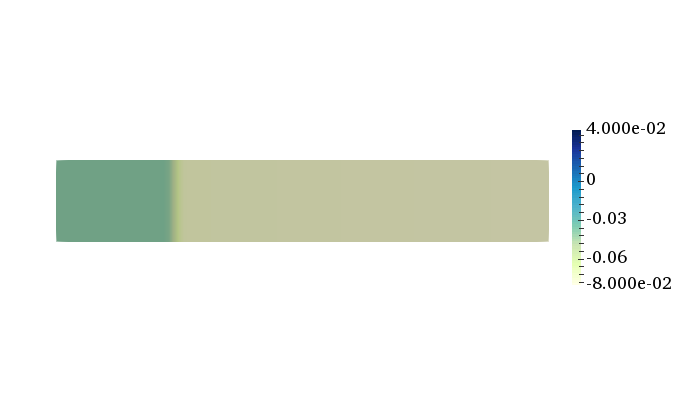
\includegraphics[trim=9cm 0cm 2cm 0cm, clip=true, width=0.9\linewidth]{v5}
%      \textbf{(c)} 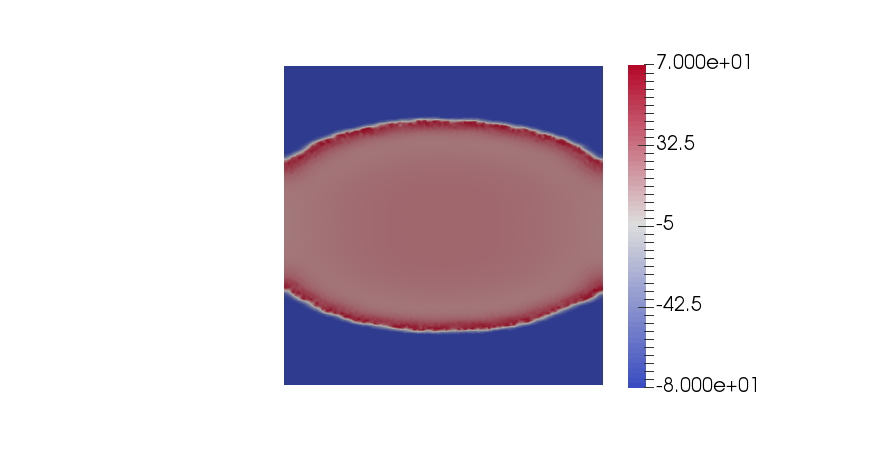
\includegraphics[trim=9cm 0cm 2cm 0cm, clip=true, width=0.9\linewidth]{v40}
%    \end{minipage}
%    \begin{minipage}{0.47\textwidth}
%  \textbf{(b)} 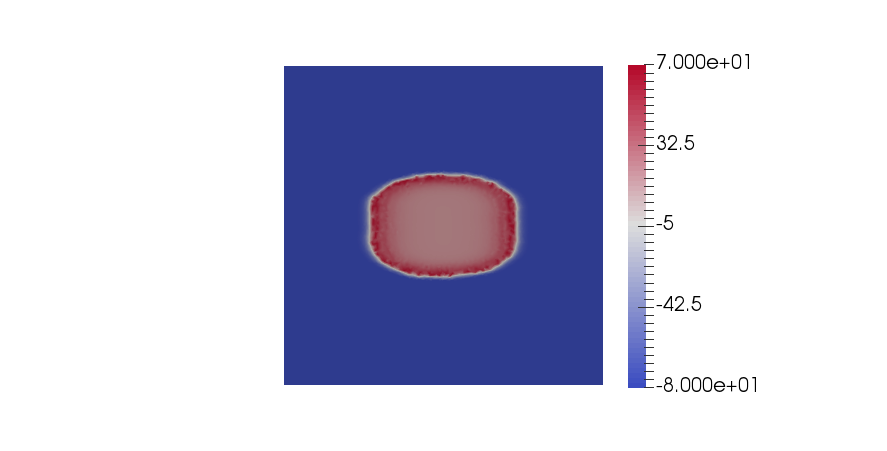
\includegraphics[trim=9cm 0cm 2cm 0cm, clip=true, width=0.9\linewidth]{v15}
%  \textbf{(d)} 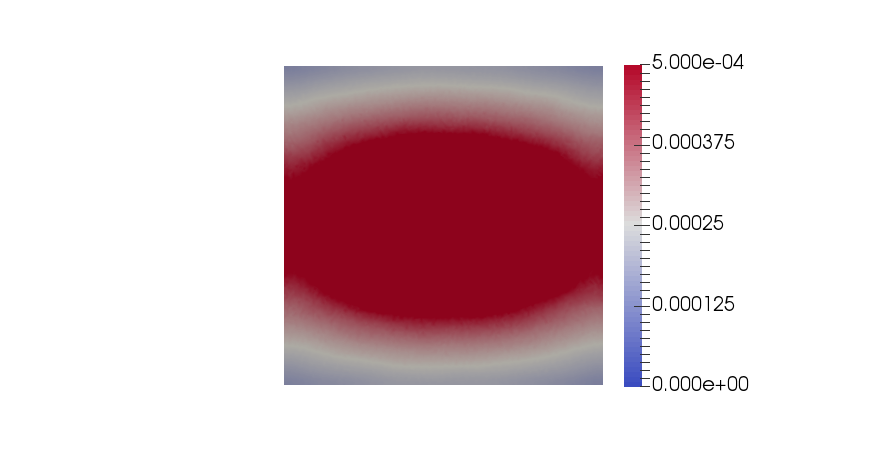
\includegraphics[trim=9cm 0cm 2cm 0cm, clip=true, width=0.9\linewidth]{Casl80}
%    \end{minipage}
%    \caption{Heat maps of $[Ca]_i$ (in $\mu$M) of our basic test case at \textbf{(a)} $t=5$ms, \textbf{(b)} $t=15$ms, \textbf{(c)} $t=40$ms and \textbf{(d)} $t=80$ms.}
%    \label{fig:2}
%\end{figure}
%%trim={<left> <lower> <right> <upper>}
%
%\begin{figure}
%   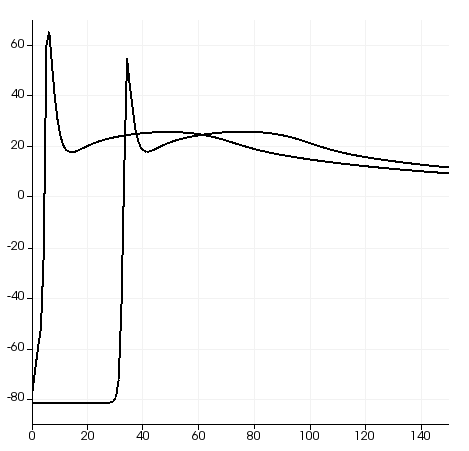
\includegraphics[width=1\linewidth]{v150} 
%    \caption{Plot of $v$ against $t$.}
%    \label{fig:3}
%\end{figure}
%
%\begin{figure}
%   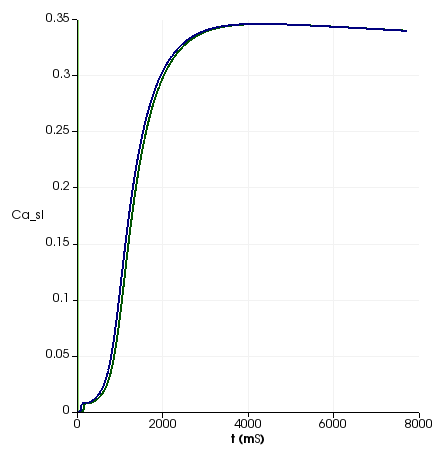
\includegraphics[width=1\linewidth]{Casl8000} 
%    \caption{Plot of $[Ca]_i$ against $t$.}
%    \label{fig:4}
%\end{figure}
%
%\section{The inverse problem} \label{The inverse problem}
%It is possible to obtain measurements $u_{\text{obs}}$ of the transmembrane potential and measurements $c_{\text{obs}}$ of the cytosolic calcium concentration $[Ca]_i$ over the whole domain $H$ at discrete points in time. With those measurements, we can estimate the value of the parameters in our model, using an adjoint-based approach.\footnote{See, for example, \cite{Gunzburger} for an introductory text in adjoint-based optimization methods.} Here, as an example, we will try to estimate the values of the $\sigma_l$ parameter from the Grandi cell model.
%We can formulate this problem as an optimisation problem: find $\sigma_l$, such that the functional
%\begin{eqnarray}
%\mathcal{J}(v, [Ca]_i, \sigma_l)= \frac{1}{N} \sum_{i=1}^{N} \frac{||v-v_{\text{obs}}(t_i)||^2_{L^2}}{||v_{\text{obs}}(t_i)||^2_{L^2}} + \frac{||[Ca]_i-[Ca]_{i\text{obs}}(t_i) ||^2_{L^2}}{||[Ca]_{i\text{obs}}(t_i) ||^2_{L^2}},\label{J}
%\end{eqnarray}
%%\begin{eqnarray} \nonumber
%%\mathcal{J}(v, c, \sigma_l)= \\ \frac{1}{N} \sum_{i=1}^{N} \int_{H}(v(\textbf{x},t_i)-\Phi(\textbf{x},t_i))^2 \: \text{d}\textbf{x} + \int_{H}\left(c(\textbf{x},t_i)-\Psi(\textbf{x},t_i)\right)^2 \: \text{d}\textbf{x},\label{J}
%%\end{eqnarray}
%is minimized, subject to the requirements that $v, c$ and $\sigma_l$ satisfy the state system of equations \eqref{eq:a}-\eqref{eq:c} and initial conditions $v(\textbf{x},0)=v_0(\textbf{x})$ and $\mathbf{s}(\mathbf{x},0)=\mathbf{s}_0(\mathbf{x})$. Here, $N$ are the number of measurements in time and $t_i$, $i=1, \dots N$ the respective moments in time.
%% https://fenicsproject.org/qa/6675/hdf-file-read-write-for-time-series
%Using cbcbeat and the dolfin-adjoint software on which it is based, we can automatically compute the total derivative of $\mathcal{J}$ with respect to the optimization parameter $\sigma_l$. We can then use the scipy optimisation algorithm \url{minimize()} -which uses the limited memory Broyden–Fletcher–Goldfarb–Shanno (BFGS) method with bound support - to find an optimal value for $\sigma_l$. We first generated some fake observed data for $\sigma_l=0.15$, from $t=0.0$ to $t=5.0$ ms, with a timestep $dt=0.05$ ms. With $\sigma_l=0.10$ as initial guess, the \url{minimize()} algorithm returned $\sigma_l=?$ after ? iterations. Similarly, we can optimize for other parameters, such as $\sigma_t$, or $g\_Na$, $g\_CaL$, $g\_K1$ or $g\_K2$ from the Grandi cell model. 
%
%%With $\sigma_t=0.01$ as initial guess and fake data created for $\sigma_t=0.02$, the \url{minimize()} algorithm converged to $\sigma_t=0.020005$ after five iterations. Optimizing for both $\sigma_l$ and $\sigma_t$, with the same initial guesses and synthetic data, gave convergence in eight iterations. The value of the functional at each iteration step was consecutively $38.6, 11.7, 10.0, 3.19, 0.89, 0.023, 0.00063, 0.0000084$ and $0.0000098$. We also looked at synthetic spatially varying $\sigma_l$ and $\sigma_t$$\ldots$

%Vragen:
%welke parameters bedoelt hij??
%-probeer fitzie
%-probeer s en s samen
%-kijken naar spatial var

%Stappenplan voor zondag:
%kijken of alleen sigma_l of sigma_t ook werkt
%kijken of c ook werkt voor taylor test
%kijken of je observaties op laatste punt kunt toevoegen
%kijken of je op meerdere punten kunt optimizen
%kijken of je dat kunt combineren met observaties

%als dat alles werkt, optimizen!! (Het echte werk, geen taylor test)

%meerdere controls, tegelijkertijd? ==> sigma_L and sigma_T

%bidomain ook proberen?
%https://docs.scipy.org/doc/scipy/reference/optimize.minimize-lbfgsb.html#optimize-minimize-lbfgsb
%minimize(fun, x0, args=(), method='L-BFGS-B', jac=None, bounds=None, tol=None, callback=None, options={'disp': None, 'maxls': 20, 'iprint': -1, 'gtol': 1e-05, 'eps': 1e-08, 'maxiter': 15000, 'ftol': 2.220446049250313e-09, 'maxcor': 10, 'maxfun': 15000})
%The iteration stops when (f^k - f^{k+1})/max{|f^k|,|f^{k+1}|,1} <= factr * eps, where eps is the machine precision, which is automatically generated by the code. Typical values for factr are: 1e12 for low accuracy; 1e7 for moderate accuracy; 10.0 for extremely high accuracy.
% Given self._vs in a correct state at t0, provide v and s (in vs) and u (in vur) in a correct state at t1. (Note that vur[0] == vs[0] only if theta = 1.0.)

%https://bitbucket.org/dolfin-adjoint/dolfin-adjoint/issues/29/adding-a-taylor-test-to-time-dependent
%
%dolfin-adjoint builds a tape of all equations and their solution variables in the background. It is the dolfin_adjoint.adj_inc_timestep function that splits this tape into multiple timelevels. If you use "u*dt[t]", dolfin_adjoint will look for the variable with the name u that was solved for at the timelevel t on the tape.

%\begin{eqnarray}
%\frac{\text{D}\mathcal{J}}{\text{D}{Gna}}=\frac{\partial \mathcal{J}}{\partial v}\frac{\partial v}{\partial Gna}
%\frac{\text{D}\mathcal{J}}{\text{D}{M_1}}=\frac{\partial \mathcal{J}}{\partial v}\frac{\partial v}{\partial M_1}+\frac{\partial \mathcal{J}}{\partial M_1}
%=\int_0^T\int_{\tilde{H}}(v-\Phi)\frac{\partial v}{\partial M_1} \: \text{d}\textbf{x}\text{dt}  + \frac{\alpha}{2}\frac{\partial\mathcal{R}}{\partial M_1} \\
%\frac{\text{D}\mathcal{J}}{\text{D}{M_2}}=\frac{\partial \mathcal{J}}{\partial v}\frac{\partial v}{\partial M_2}+\frac{\partial \mathcal{J}}{\partial M_2}
%=\int_0^T\int_{\tilde{H}}(v-\Phi)\frac{\partial v}{\partial M_2} \: \text{d}\textbf{x}\text{dt}  + \frac{\alpha}{2}\frac{\partial\mathcal{R}}{\partial M_2}. \label{totdef}
%\end{eqnarray}

%We will use an adjoint-based approach.\footnote{See, for example, \cite{Gunzburger} for an introductory text in adjoint-based optimization methods. See \cite{Yang} for an adjoint-based approach for the estimation of the cardiac conductivity paramters of the bidomain equations.} Consider the Lagrangian functional:
%\begin{eqnarray} 
%% L
%\mathcal{L}(v, \mathbf{M}, \mathbf{s}, \lambda, \boldsymbol{\mu})=
%% J
%\mathcal{J}(v, \mathbf{M}) 
%\nonumber \\
%% \lambda
%-\int_0^T\int_{H} \lambda \left(\frac{\partial v}{\partial t} + I_{ion}(v,\mathbf{s}) -\nabla \cdot(\mathbf{M}\nabla v) - I_s)\right) \:\text{d}\textbf{x}\text{dt} 
%\nonumber \\
%% mu
%-\int_0^T \int_{H} \boldsymbol{\mu} \cdot \left(\frac{\partial \mathbf{s}}{\partial t}- \mathbf{F}(\mathbf{s},v)\right) \:\text{d}\textbf{x}\text{dt}.
%\end{eqnarray}
%Setting the first variation with respect to the state variables $v$ and $\mathbf{s}$ equal to zero yields the adjoint system:
%\begin{eqnarray} \label{ad1}
%\frac{\partial \lambda}{\partial t} + \lambda \frac{\partial I_{ion}}{\partial v} -\nabla \cdot(\mathbf{M}\nabla \lambda) + \boldsymbol{\mu} \cdot \frac{\partial \mathbf{F}}{\partial v}
% = v-\Phi \qquad &\text{on}& \qquad \tilde{H}, \\\label{ad2}
%\frac{\partial \lambda}{\partial t} + \lambda \frac{\partial I_{ion}}{\partial v} -\nabla \cdot(\mathbf{M}\nabla \lambda) + \boldsymbol{\mu} \cdot \frac{\partial \mathbf{F}}{\partial v} = 0 \qquad &\text{on}& \qquad H-\tilde{H}, \\\label{ad3}
%\lambda\frac{\partial I_{ion}}{\partial \mathbf{s}} + 
%\frac{\partial\boldsymbol{\mu}}{\partial{dt}}-\boldsymbol{\mu}\cdot \frac{\partial\mathbf{F}}{\partial \mathbf{s}} = 0\qquad &\text{on}& \qquad H,
%\end{eqnarray}
%with terminal conditions $\lambda(\textbf{x},T)=0$ and $\boldsymbol{\mu}(\mathbf{x},T)=0$. Plugging equations \eqref{ad1}-\eqref{ad2} into equation \eqref{totdef} yields:
%\begin{eqnarray}
%\frac{\text{D}\mathcal{J}}{\text{D}\mathbf{M}}
%=\int_0^T\int_{{H}}\left(\frac{\partial \lambda}{\partial t} + \lambda \frac{\partial I_{ion}}{\partial v} -\nabla \cdot(\mathbf{M}\nabla \lambda) + \boldsymbol{\mu} \cdot \frac{\partial \mathbf{F}}{\partial v}\right)\frac{\partial v}{\partial\mathbf{M}} \: \text{d}\textbf{x}\text{dt} + \frac{\alpha}{2}\frac{\partial\mathcal{R}}{\partial \mathbf{M}}. 
%\end{eqnarray}
%We integrate by parts:
%\begin{eqnarray} \nonumber
%\frac{\text{D}\mathcal{J}}{\text{D}\sigma}
%=\int_0^T\int_{{H_i}}\nabla \cdot \sigma_i \nabla \left(\frac{\partial u_i}{\partial\sigma}\right)\xi \: \text{d}\textbf{x}\text{dt}  +\int_0^T\int_{{H_e}}\nabla \cdot \sigma_e \nabla \left(\frac{\partial u_e}{\partial\sigma}\right)\mu \: \text{d}\textbf{x}\text{dt} \\ \nonumber
%+ \int_0^T\int_{{\Gamma}} \left(\frac{\partial u_i}{\partial\sigma}\right)n_i \cdot \sigma_i \nabla \xi + \left(\frac{\partial u_e}{\partial\sigma}\right)n_e \cdot \sigma_e \nabla \mu 
%\: \text{d}\textbf{s}\text{dt} \\ \nonumber
%-\int_0^T\int_{{\Gamma}}
% \xi \left(n_i \cdot \sigma_i \nabla \left(\frac{\partial u_i}{\partial\sigma}\right)\right) + \mu \left(n_e \cdot \sigma_e \nabla \left(\frac{\partial u_e}{\partial\sigma}\right)\right) \: \text{d}\textbf{s}\text{dt} \\
%+ \int_0^T\int_{{\Gamma}}\left(\theta -C_m \frac{\partial \rho}{\partial t} +\rho \frac{\partial{f}}{\partial u_m}-\boldsymbol{\tau}\cdot \frac{\partial\mathbf{g}}{\partial u_m}\right)\frac{\partial u_m}{\partial\sigma} \: \text{d}\textbf{s}\text{dt} + \frac{\alpha}{2}\frac{\partial\mathcal{R}}{\partial \sigma}. 
%\end{eqnarray}
%Now, we differentiate our state equation system \eqref{3}-\eqref{7b} with respect to $\sigma_i$ and $\sigma_e$:
%\begin{eqnarray}
%\frac{\partial}{\partial}
%\end{eqnarray}
%\begin{color}{red} \end{color}
%\section*{Appendix A}
%To derive the adjoint system as given by equations \eqref{ad1}-\eqref{adz}, with terminal conditions $\rho(\textbf{s},T)=0$ and $\boldsymbol{r}(\mathbf{s},T)=0$, we set the first variation of the Lagrangian with respect to the state parameters $u_i, u_e, u_m, I_m$ and $\mathbf{w}$ equal to zero and integrate by parts. Setting the first variation with respect to $u_i$ equal to zero gives us:
%\begin{eqnarray} \nonumber
%\int_0^T \int_{\tilde{H_i}}\tilde{u}_i(u_i-\Phi_i)\: \text{d}\textbf{x}\text{dt} = \\
%\int_0^T \int_{H_i}\xi(\nabla \cdot \sigma_i \nabla \tilde{u}_i)\: \text{d}\textbf{x}\text{dt} +  \int_0^T \int_{\Gamma}-\theta \tilde{u}_i + (\zeta + \eta)(n_i \cdot \sigma_i \nabla \tilde{u}_i)\: \text{d}\textbf{s}\text{dt},
%\end{eqnarray}
%for arbitrary variations $\tilde{u}_i$ of $u_i$.
%We integrate by parts:
%\begin{eqnarray} \nonumber
%\int_0^T \int_{\tilde{H_i}}\tilde{u}_i(u_i-\Phi_i)\: \text{d}\textbf{x}\text{dt} = \int_0^T \int_{H_i}\tilde{u}_i(\nabla \cdot \sigma_i \nabla \xi)\: \text{d}\textbf{x}\text{dt} \\ 
%+  \int_0^T \int_{\Gamma}-\theta \tilde{u}_i + (\zeta + \eta +\xi)(n_i \cdot \sigma_i \nabla \tilde{u}_i) - \tilde{u}_i (n_i \cdot \sigma_i \nabla \xi)\: \text{d}\textbf{s}\text{dt}.
%\end{eqnarray}
%Since variations in $\tilde{u}_i$ are arbitrary, we obtain:
%\begin{eqnarray}
%\nabla \cdot \sigma_i \nabla \xi = u_i-\Phi_i \qquad &\text{on}& \qquad \tilde{H_i}, \\
%\nabla \cdot \sigma_i \nabla \xi = 0 \qquad &\text{on}& \qquad H-\tilde{H_i}, \\
%\zeta+\eta+\xi=0 \qquad &\text{on}& \qquad {\Gamma}, \\
%\theta=-n_i \cdot \sigma_i \nabla \xi \qquad &\text{on}& \qquad {\Gamma}.
%\end{eqnarray}
%Similarly, setting the first variation with respect to$u_e$ equal to zero gives us:
%\begin{eqnarray} \nonumber
%\int_0^T \int_{\tilde{H_e}}\tilde{u}_e(u_e-\Phi_e)\: \text{d}\textbf{x}\text{dt} =
%\int_0^T \int_{H_e}\mu(\nabla \cdot \sigma_e \nabla \tilde{u}_e)\: \text{d}\textbf{x}\text{dt} \\
%+\int_0^T \int_{\delta H_e}\tilde{u_e}\nu\: \text{d}\textbf{s}\text{dt}+  \int_0^T \int_{\Gamma}\theta \tilde{u}_e + \zeta(n_e \cdot \sigma_e \nabla \tilde{u}_e)\: \text{d}\textbf{s}\text{dt},
%\end{eqnarray}
%for arbitrary variations $\tilde{u}_e$ of $u_e$.
%We integrate by parts:
%\begin{eqnarray} \nonumber
%\int_0^T \int_{\tilde{H}}\tilde{u}_e(u_e-\Phi_e)\: \text{d}\textbf{x}\text{dt} = \int_0^T \int_{H_e}\tilde{u}_e(\nabla \cdot \sigma_e \nabla \mu)\: \text{d}\textbf{x}\text{dt} \\ \nonumber +\int_0^T \int_{\deltaH_e} \mu(n_e \cdot \sigma_e \nabla \tilde{u}_e) + \tilde{u}_e (\nu - n_e \cdot \sigma_e \nabla \mu)\: \text{d}\textbf{s}\text{dt} \\
%+  \int_0^T \int_{\Gamma}\theta \tilde{u}_e + (\zeta +\mu)(n_e \cdot \sigma_e \nabla \tilde{u}_e) - \tilde{u}_e (n_e \cdot \sigma_e \nabla \mu)\: \text{d}\textbf{s}\text{dt}.
%\end{eqnarray}
%Since variations in $\tilde{u}_e$ are arbitrary, we obtain:
%\begin{eqnarray}
%\nabla \cdot \sigma_e \nabla \mu = u_e-\Phi_e \qquad &\text{on}& \qquad \tilde{H_e}, \\
%\nabla \cdot \sigma_e \nabla \mu = 0 \qquad &\text{on}& \qquad H-\tilde{H_e}, \\
%\zeta+\mu=0 \qquad &\text{on}& \qquad {\Gamma}, \\
%\theta=n_e \cdot \sigma_e \nabla \mu \qquad &\text{on}& \qquad {\Gamma} \\
%\nu=n_e \cdot \sigma_e \nabla \mu \qquad &\text{on}& \qquad {\delta H}\\
%\mu=0 \qquad &\text{on}& \qquad {\delta H}.
%\end{eqnarray}
%Setting the first variation with respect to $u_m$ equal to zero is equivalent to:
%\begin{eqnarray} \nonumber
%\int_0^T \int_{\tilde{\Gamma}}\tilde{u}_m(u_m-\Phi_m)\: \text{d}\textbf{s}\text{dt} = \\ \nonumber
%\int_0^T \int_{\Gamma}\tilde{u}_m \theta + \rho\left(C_m \frac{\partial \tilde{u}_m}{\partial t} + \frac{\partial f}{\partial {u}_m}\tilde{u}_m\right)-\boldsymbol{\tau}\cdot \frac{\partial\mathbf{g}}{\partial {u}_m}\tilde{u}_m \: \text{d}\textbf{s}\text{dt}\\
%+\int_\Gamma \tilde{u}_m(\mathbf{s},0)\kappa(\mathbf{s},0) \: \text{d}\textbf{s},
%\end{eqnarray}
%for arbitrary variations $\tilde{u}_m$ of $u_m$.
%We integrate by parts:
%\begin{eqnarray} \nonumber
%\int_0^T \int_{\tilde{\Gamma}}\tilde{u}_m(u_m-\Phi_m)\: \text{d}\textbf{s}\text{dt} = \\ \nonumber
%\int_0^T \int_{\Gamma} \tilde{u}_m \theta- \tilde{u}_m C_m \frac{\partial \rho}{\partial t} + \rho\frac{\partial{f}}{\partial {u}_m}\tilde{u}_m-\boldsymbol{\tau}\cdot \frac{\partial\mathbf{g}}{\partial {u}_m}\tilde{u}_m \: \text{d}\textbf{s}\text{dt} \\ +\int_\Gamma \tilde{u}_m(\mathbf{s},0)\kappa(\mathbf{s},0) + C_m \left(\rho(\mathbf{s},T) \tilde{u}_m(\mathbf{s},T)- \rho(\mathbf{s},0) \tilde{u}_m(\mathbf{s},0)
%\right)\: \text{d}\textbf{s}.
%\end{eqnarray}
%Since variations in $\tilde{u}_m$ are arbitrary, we obtain:
%\begin{eqnarray} \nonumber
%\theta - C_m \frac{\partial \rho}{\partial t} +\rho \frac{\partial{f}}{\partial u_m}-\boldsymbol{\tau}\cdot \frac{\partial\mathbf{g}}{\partial u_m}= u_m-\Phi_m \qquad &\text{on}& \qquad \tilde{\Gamma}, \\
%\theta - C_m \frac{\partial \rho}{\partial t} +\rho \frac{\partial{f}}{\partial u_m}-\boldsymbol{\tau}\cdot \frac{\partial\mathbf{g}}{\partial u_m}= 0 \qquad &\text{on}& \qquad \Gamma-\tilde{\Gamma},
%\end{eqnarray}
%$C_m\rho(\textbf{s},0)=\kappa(\textbf{s},0)$ and $\rho(\textbf{s},T)=0$.
%Setting the first variation with respect to $I_m$ equal to zero is equivalent to:
%\begin{eqnarray} 
%\int_0^T \int_{\tilde{\Gamma}}(\eta+\rho)\tilde{I}_m\: \text{d}\textbf{s}\text{dt} = 0,
%\end{eqnarray}
%for arbitrary variations $\tilde{I}_m$ of $I_m$. Since variations in $\tilde{I}_m$ are arbitrary, we obtain:
%\begin{eqnarray}
%\eta=-\rho \qquad &\text{on}& \qquad \tilde{\Gamma}.
%\end{eqnarray}
%Finally, setting the first variation with respect to $\mathbf{w}$ equal to zero gives us:
%\begin{eqnarray} 
%\int_0^T \int_{{\Gamma}}\rho\frac{\partial f}{\partial \mathbf{w}}\tilde{\mathbf{w}} + \boldsymbol{\tau} \cdot \left( \frac{\text{d}\mathbf{\tilde{w}}}{\text{dt}}- \frac{\partial \mathbf{g}}{\partial \mathbf{w}}\tilde{\mathbf{w}}\right)\: \text{d}\textbf{x}\text{dt} + \int_{{\Gamma}}\boldsymbol{\lambda}(\mathbf{s},0)\cdot \mathbf{\tilde{w}(\mathbf{s},0)}\: \text{d}\textbf{x}= 0,
%\end{eqnarray}
%for arbitrary variations $\tilde{\mathbf{w}}$ of $\mathbf{w}$.
%We integrate by parts:
%\begin{eqnarray} \nonumber
%\int_0^T \int_{{\Gamma}}\rho\frac{\partial f}{\partial \mathbf{w}}\tilde{\mathbf{w}} - \mathbf{\tilde{w}} \cdot \frac{\text{d}\boldsymbol{\tau}}{\text{dt}}- \boldsymbol{\tau} \cdot\frac{\partial \mathbf{g}}{\partial \mathbf{w}}\tilde{\mathbf{w}}\: \text{d}\textbf{x}\text{dt} \\ +\int_{{\Gamma}}\boldsymbol{\tau}(\mathbf{s},T)\cdot\mathbf{\tilde{w}}(\mathbf{s},T) - \boldsymbol{\tau}(\mathbf{s},0)\cdot\mathbf{\tilde{w}}(\mathbf{s},0)+ \boldsymbol{\lambda}(\mathbf{s},0)\cdot \mathbf{\tilde{w}(\mathbf{s},0)}\: \text{d}\textbf{x}= 0.
%\end{eqnarray}
%Since variations in $\tilde{\mathbf{w}}$ are arbitrary, we obtain:
%\begin{eqnarray}
%\frac{\text{d}\boldsymbol{\tau}}{\text{dt}}-\rho \frac{\partial{f}}{\partial \mathbf{w}}+\boldsymbol{\tau}\cdot \frac{\partial\mathbf{g}}{\partial \mathbf{w}} = 0\qquad &\text{on}& \qquad \Gamma,
%\end{eqnarray}
%$\boldsymbol{\tau}(\textbf{s},0)=\boldsymbol{\lambda}(\textbf{s},0)$ and $\boldsymbol{\tau}(\textbf{s},T)=0$.

\begin{thebibliography}{99}
%\bibitem{Grandi} Grandi, Pasqualini, Puglisi, \& Bers. (2009). A Novel Computational Model of the Human Ventricular Action Potential and Ca transient. \textit{Biophysical Journal, 96}(3), 664a-665a.
%\bibitem{Gunzburger} Gunzburger, M. (2003). \textit{Perspectives in flow control and optimization} (Advances in design and control). Philadelphia, Pa.: SIAM.
%\bibitem{Roth} Sepulveda, Roth, \& Wikswo. (1989). Current injection into a two-dimensional anisotropic bidomain. \textit{Biophysical Journal, 55}(5), 987-999.
%\bibitem{Plonsey1882} Plonsey, R., \& Barr, R. (1982). The Four-Electrode Resistivity Technique as Applied to Cardiac Muscle. \textit{Biomedical Engineering, IEEE Transactions on, BME-29}(7), 541-546.
%\bibitem{Plonsey1984} Barr, \& Plonsey. (1984). Propagation of excitation in idealized anisotropic two-dimensional tissue. \textit{Biophysical Journal, 45}(6), 1191-1202.
%\bibitem{fenics} \url{fenicsproject.org}
%\bibitem{dolfin-adjoint} \url{www.dolfin-adjoint.org}
%\bibitem{cbcbeat} \url{bitbucket.org/meg/cbcbeat}
\bibitem{Blazeski} Blazeski, A., Zhu, R., Hunter, D. W., Weinberg, S. H., Boheler, K. R., Zambidis, E. T., \& Tung, L. (2012). Electrophysiological and contractile function of cardiomyocytes derived from human embryonic stem cells. \textit{Progress in Biophysics and Molecular Biology, 110}(0), 178–195.
\bibitem{Denning2016} Denning, C., Borgdorff, V., Crutchley, J., Firth, K. S., George, V., Kalra, S., \ldots Prodanov, L. (2016). Cardiomyocytes from human pluripotent stem cells: from laboratory curiosity to industrial biomedical platform. \textit{Biochimica et Biophysica Acta (BBA)-Molecular Cell Research, 1863}(7), 1728-1748.
\bibitem{Lee2012} Lee, P., Klos, M., Bollensdorff, C., Hou, L., Ewart, P., Kamp, T. J., \ldots Jalife, J. (2012). Simultaneous Voltage and Calcium Mapping of Genetically Purified Human Induced Pluripotent Stem Cell–Derived Cardiac Myocyte MonolayersNovelty and Significance. \textit{Circulation research, 110}(12), 1556-1563.
\bibitem{Leyton2014} Leyton-Mange, J. S., Mills, R. W., Macri, V. S., Jang, M. Y., Butte, F. N., Ellinor, P. T., \& Milan, D. J. (2014). Rapid cellular phenotyping of human pluripotent stem cell-derived cardiomyocytes using a genetically encoded fluorescent voltage sensor. \textit{Stem Cell Reports, 2}(2), 163-170.
\bibitem{Ma2011} Ma, J., Guo, L., Fiene, S., Anson, B., Thomson, J., Kamp, T., \ldots January, C. (2011). High purity human-induced pluripotent stem cell-derived cardiomyocytes: Electrophysiological properties of action potentials and ionic currents. \textit{American Journal of Physiology. Heart and Circulatory Physiology, 301}(5), H2006-17.
\bibitem{KeenerI} Keener, J. P., \& Sneyd, J. (2009). \textit{Mathematical physiology (Vol. I)}. New York: Springer.
\bibitem{KeenerII} Keener, J. P., \& Sneyd, J. (2009). \textit{Mathematical physiology (Vol. II)}. New York: Springer.
\bibitem{Paci2013} Paci, M., Hyttinen, J., Aalto-Set\"al\"a, K., \& Severi, S. (2013). Computational models of ventricular-and atrial-like human induced pluripotent stem cell derived cardiomyocytes. \textit{Annals of biomedical engineering, 41}(11), 2334-2348.
\bibitem{Rajamohan2013} Rajamohan, D., Matsa, E., Kalra, S., Crutchley, J., Patel, A., George, V., \& Denning, C. (2013). Current status of drug screening and disease modelling in human pluripotent stem cells. \textit{Bioessays, 35}(3), 281-298.
\bibitem{Sallam2016} Sala, L., Bellin, M., \& Mummery, C. (2016). Integrating cardiomyocytes from human pluripotent stem cells in safety pharmacology: Has the time come?: Implementation of hiPSC-CMs in cardiotoxicity. \textit{British Journal of Pharmacology}.
\bibitem{Takahashi2007} Takahashi, K., Tanabe, K., Ohnuki, M., Narita, M., Ichisaka, T., Tomoda, K., \& Yamanaka, S. (2007). Induction of pluripotent stem cells from adult human fibroblasts by defined factors. \textit{cell, 131}(5), 861-872.
\bibitem{Zhu2016} Zhu, R., Millrod, M. A., Zambidis, E. T., \& Tung, L. (2016). Variability of action potentials within and among cardiac cell clusters derived from human embryonic stem cells. \textit{Scientific reports, 6}, 18544.
\bibitem{cellml} \url{models.cellml.org/electrophysiology}
\end{thebibliography}
\end{document}